\chapter{The Standard Model of Particle Physics}

Ever since Democritus' philosophy of atomism, one of the driving desires behind mankind's advancements in the fields of natural science has been to reduce reality to its basic components.

[...], this chapter explores the theoretical framework for the rest of thesis, introducing key concepts such as \textit{spin}, \textit{helicity} and the importance of \textit{angular distributions} of decay products.

\section{Elementary particles}
\begin{figure}[t!]
	\centering
	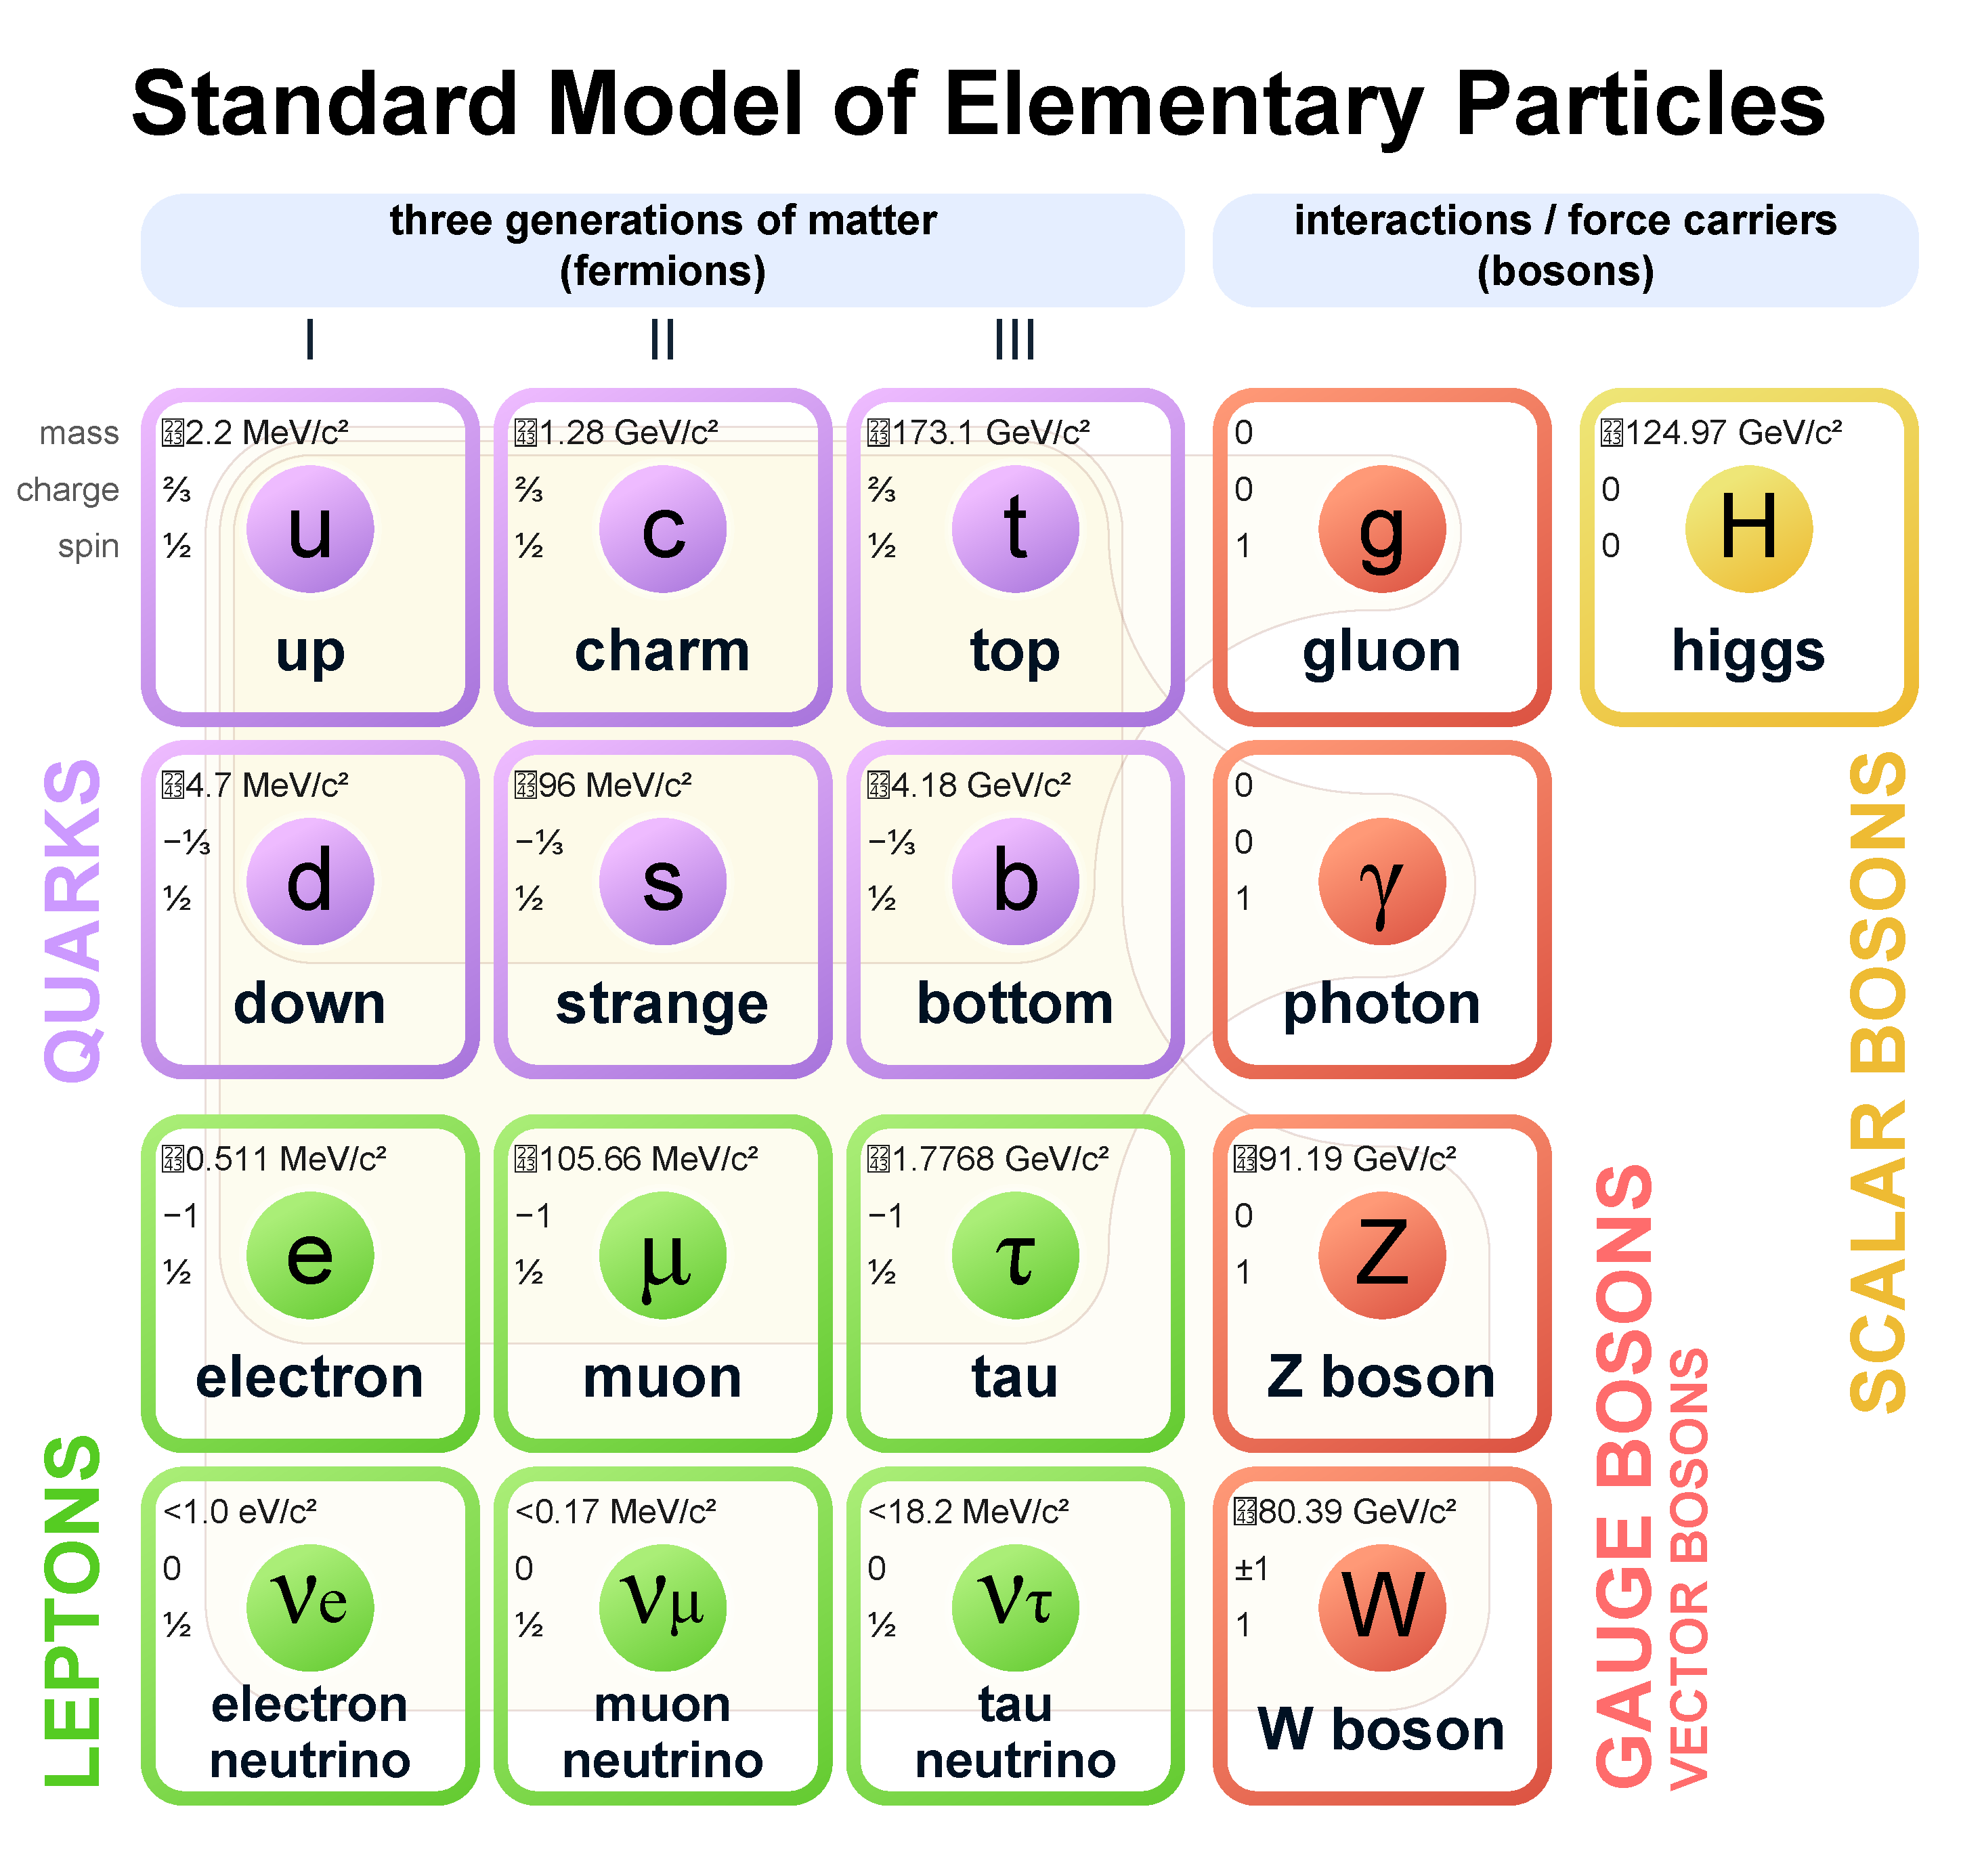
\includegraphics[scale=0.15]{graphics/01-standard_model/Standard_Model_of_Elementary_Particles.pdf}
	\caption[Currently known Standard Model elementary particles.]{The seventeen currently known elementary particles of the Standard Model. Antiparticles are not depicted.}
	\label{fig:particle_zoo}
\end{figure}

Intuitively, a particle is said to be \textit{elementary} when no substructure can be probed. 
A century of efforts in the fields of nuclear, quantum, and high energy physics has whittled down the spectrum of matter to just seventeen unique fundamental particles, colloquially known as the \textit{particle zoo} and depicted in Figure \ref{fig:particle_zoo}.

Each particle is joined by an \textit{antimatter particle} (\textit{antiparticle} for short), a companion of opposite charge identified by the prefix \textit{anti-}, e.g. antimuon for the muon; the only exception to this naming convention is the electron, whose antiparticle, for historical reasons, is known as positron.
While often omitted for the sake of brevity, antiparticles are elementary particles in every respect, distinct from their partners (bar the neutral gauge bosons, which are their own antiparticles) and related to them through the transformation of \textit{charge conjugation}.

\subsection{Leptons}
Leptons are fermions (half-integer spin particles) not sensitive to the strong nuclear interaction. There are currently six \textit{flavours} of leptons grouped in three generations: each generation is comprised of a \textit{charged} lepton (electron, muon, tauon) and a \textit{neutral} lepton (electron neutrino, muon neutrino, tauon neutrino).

All charged leptons have a charge of $-q_e$, where $q_e$ is defined as the \textit{elementary positive charge}, and their mass ranges from $\approx \SI{0.5}{MeV}$ for the electron to over $\SI{1.7}{GeV}$ for the tauon. By contrast, as the names suggest, all neutrinos are electrically neutral and are assumed massless in the Standard Model\footnote{The observation of flavour oscillation in solar neutrinos shows that neutrinos do in fact have non-zero, albeit very small, mass. This discrepancy is considered one of the major puzzles of the Standard Model.}; this implies that their only meaningful interactions happen through the weak nuclear force, which grants them their characteristic evasiveness to most particle detectors.


\subsection{Quarks}
Much like leptons, quarks are also fermions existing in three generations. The main difference from the former category is that quarks, besides interacting through weak and electromagnetic forces, are also susceptible to the strong nuclear forces; this allows them to bind together in composite states known as \textit{hadrons}, which are classified as \textit{baryons} (states of three quarks) and \textit{mesons} (states of one quark and one antiquark).

Quarks can be classified as \textit{up-type} (up, charm and top quarks) and \textit{down-type} (down, strange and bottom quarks): up-type quarks have a fractionary charge of $+\frac{2}{3} q_e$, whereas down-type quarks have a charge of $-\frac{1}{3} q_e$. All quarks also have one of three \textit{color} charges (red, green or blue), while antiquarks similarly have one of three \textit{anti-color} charges (antired, antigreen or antiblue). A combination of all three colors/anti-colors or a combination of a color and its matching anticolor produces \textit{colorless} particles, a property of all observed quark composite states.

[Mescolamento dei sapori.]

\begin{equation}
	\begin{pmatrix}
		d' \\
		s' \\
		b'
	\end{pmatrix}
	=
	\begin{pmatrix}
		V_{ud} & V_{us} & V_{ub} \\
		V_{cd} & V_{cs} & V_{cb} \\
		V_{td} & V_{ts} & V_{tb}
	\end{pmatrix}
	\begin{pmatrix}
		d \\
		s \\
		b
	\end{pmatrix}
	\label{eq:CKM_matrix}
\end{equation}

Unlike leptons, quarks are impossible to observe directly: according to the phenomenon of \textit{color confinement}, the energy of the interaction field between two color charges being pulled apart increases with their distance until it becomes high enough to create a quark-antiquark pair.
This process of \textit{fragmentation} develops many times over in such a way that the final observable state is entirely composed of colorless particles.
For this reason, high energy physics experiments such as LHCb do not detect free quarks, instead observing cone-shaped streams of hadrons known as \textit{hadronic jets}.

\subsection{Gauge bosons and fundamental interactions}
The fundamental forces driving the interactions between elementary particles are introduced in the Standard Model via the so-called \textit{gauge principle}.

[Gruppo di simmetria, principio di gauge, QCD e teoria elettrodebole.]

There is no gauge boson associated to the fourth known fundamental force, gravity.
Since every attempt to reconcile the general theory of relativity with quantum mechanics has failed so far, gravity is presently excluded from the Standard Model; this doesn't affect SM predictions at the subatomic level on account of the remarkably low intensity of said force, over 30 orders of magnitude lower than the weak interaction.

\subsection{The Higgs boson}
[Rottura spontanea della simmetria.]

\section{Spin}
[Spin ed EM dipole.]

\section{Discrete symmetries}
[CPT, violazione di CP.]

\section{Helicity formalism}
[Il Richman.]